\chapter{The CMS Experiment and the CERN LHC}

\section{The LHC}

\subsection{LHC Pre-Acceleration}

\subsection{LHC Acceleration}

\section{The CMS Experiment}

point 5
general purpose
    designed for Higgs discovery
    measure energy and momentum of particle
    tracker for momentum
    ECAL / HCAL for energy
    muon spectrometer for muon momentum
    magnet
    hermetic
40 MHz - high speed electronics capable of operating in close synchronization
trigger, L1, HLT

CMS IMAGE

XXXXXXXXXXXXXXXXXXXXXXXXXXXXXXXXX

The central feature of the CMS apparatus is a superconducting solenoid of 6 meters internal diameter, providing a magnetic field of 3.8 Tesla. Within the solenoid volume, there are a silicon pixel and strip tracker, a lead tungstate crystal electromagnetic calorimeter (ECAL), and a brass and scintillator hadron calorimeter (HCAL), each composed of a barrel and two endcap sections. Forward calorimeters extend the pseudorapidity coverage provided by the barrel and endcap detectors. Muons are detected in gas-ionization chambers embedded in the steel flux-return yoke outside the solenoid.

Events of interest are selected using a two-tiered trigger system~\cite{Khachatryan:2016bia}. The first level (L1), composed of custom hardware processors, uses information from the calorimeters and muon detectors to select events at a rate of around 100 kHz within a time interval of less than 4 microseconds. The second level, known as the high-level trigger (HLT), consists of a farm of processors running a version of the full event reconstruction software optimized for fast processing, and reduces the event rate to about 1 kHz before data storage.

Significant upgrades of the L1 trigger during the first long shutdown of the LHC have benefitted this analysis, especially in the $\tauh\tauh$ channel. These upgrades improved the $\tauh$ identification at L1 by giving more flexibility to object isolation, allowing new techniques to suppress the contribution from additional $\Pp\Pp$ interactions per bunch
crossing, and to reconstruct the L1 $\tauh$ object in a fiducial region that matches more closely that of a true hadronic $\Pgt$ decay. The flexibility is achieved by employing high bandwidth optical links for data communication and large field-programmable gate arrays (FPGAs) for data processing.

A more detailed description of the CMS detector, together with a definition of the coordinate system used and the relevant kinematic variables, can be found in Ref.~\cite{Chatrchyan:2008zzk}.

\subsection{Geometry}
CMS center = (0,0,0)
+x, lhc center
+y, vertical
+z, clockwise

quasicylindrical coordinates (pt,eta,phi)
\begin{equation}
\pt \equiv \sqrt{p^{2}_{x} + p^{2}_{y}}
\end{equation}
\begin{equation}
\eta \equiv -ln\bigg[\tan\bigg(\frac{\theta}{2}\bigg)\bigg]
\end{equation}
phi is defined in the x-y plane

\subsection{Magnet}
\subsection{Inner Tracking System}

The tracker measures the pT of charged hadrons at normal incidence with a resolution of 1\% for pT $<$ 20 GeV

\begin{figure*}[htbp]
\centering
     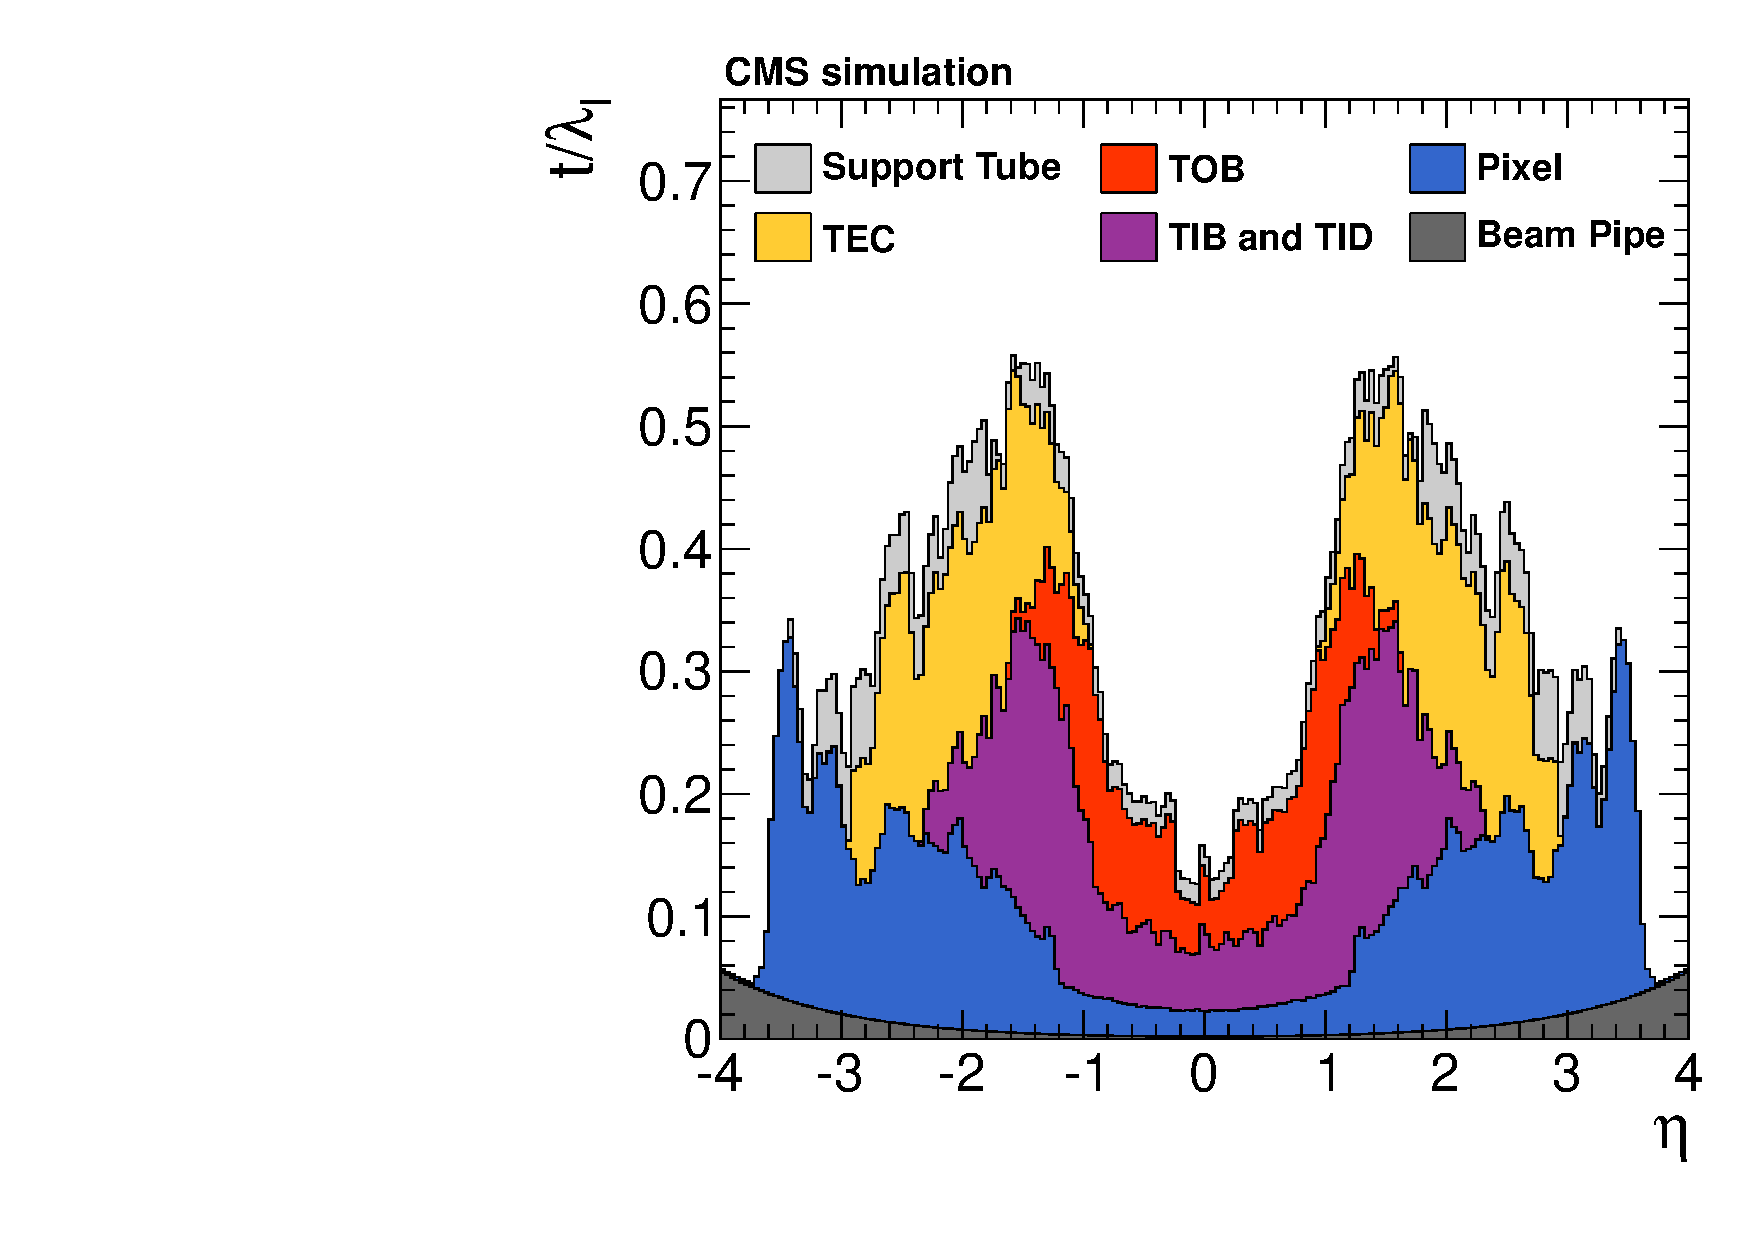
\includegraphics[width=0.4\textwidth]{cms_and_lhc/plots/cms_tracker_thickness_radiationL.pdf}
     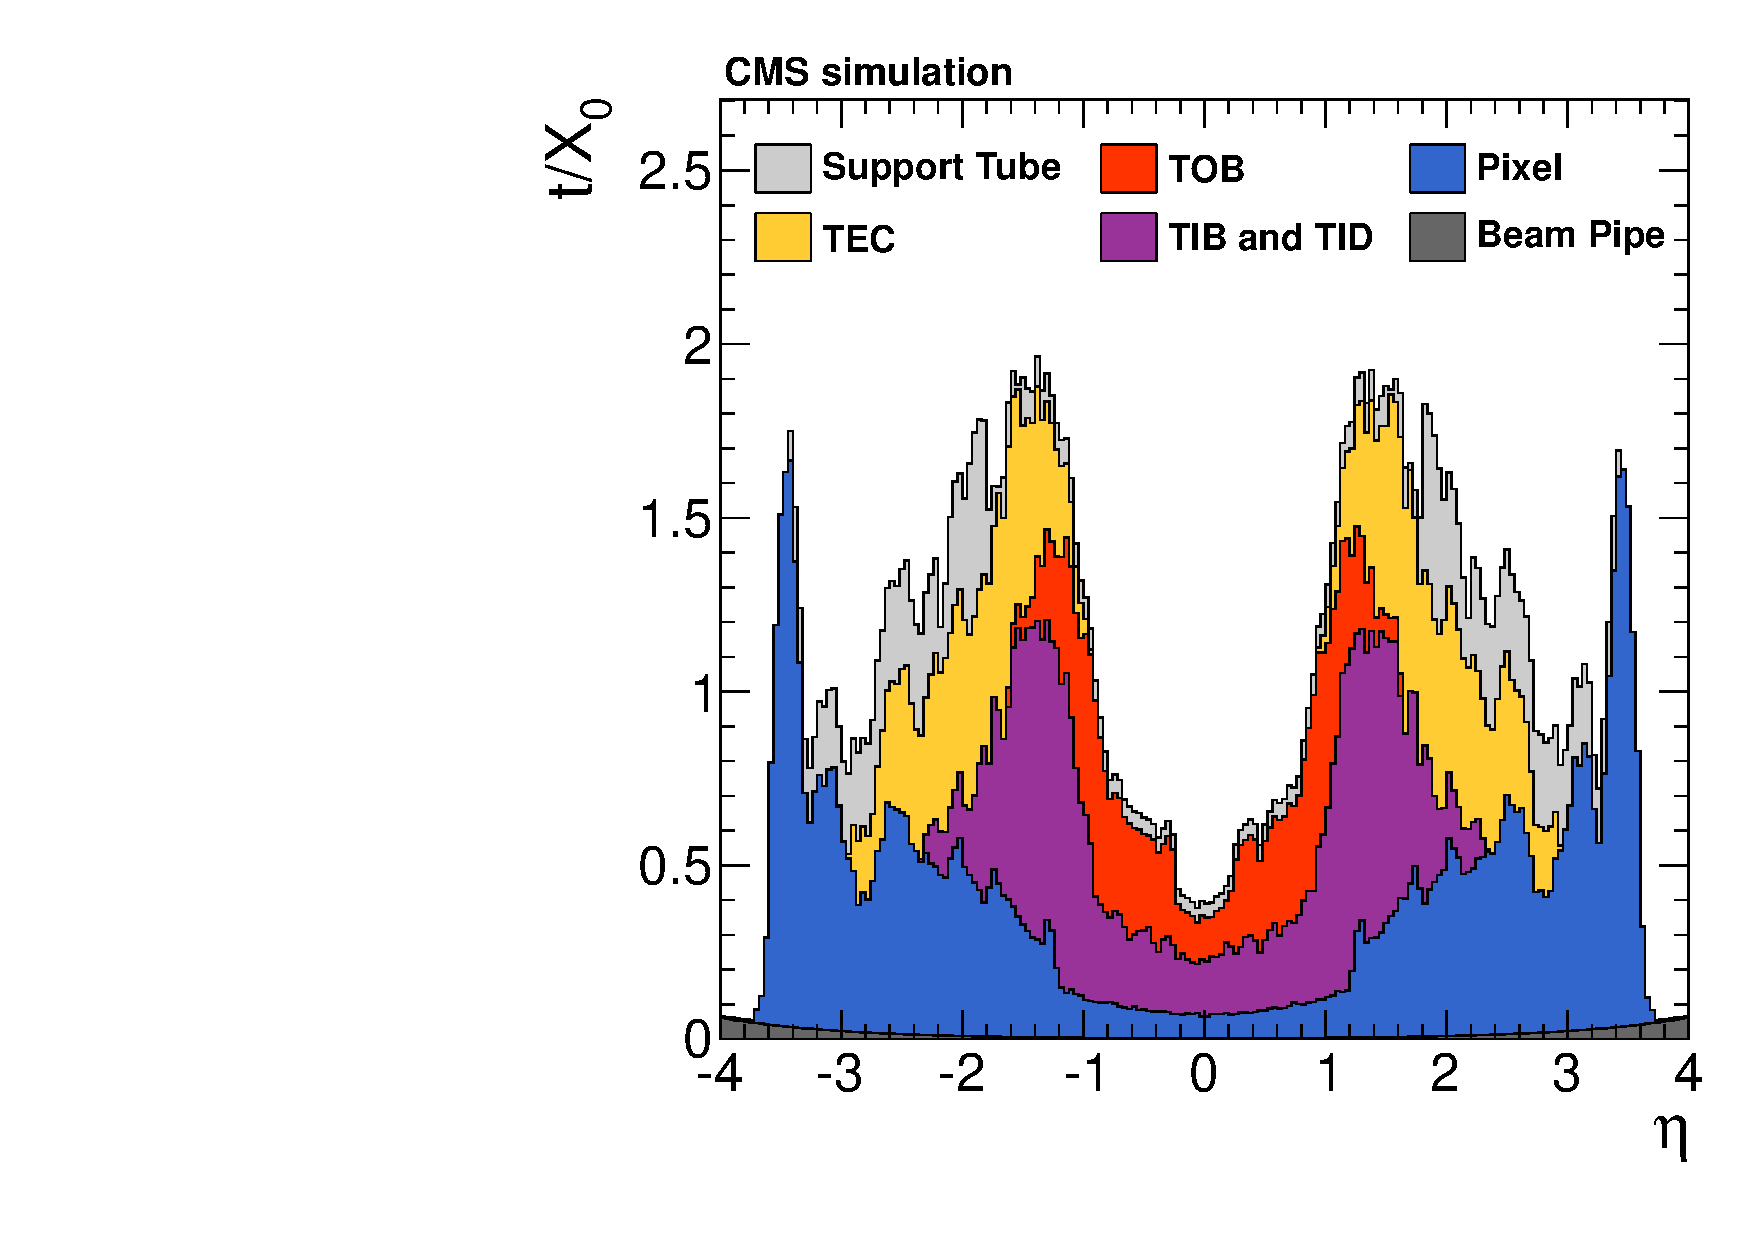
\includegraphics[width=0.4\textwidth]{cms_and_lhc/plots/cms_tracker_thickness_interactionL.pdf}
     \caption{
Total thickness t of the inner tracker material expressed in units of interaction lengths $\lambda_{l}$ (left) and radiation lengths X0 (right), as a function of the pseudorapidity $\eta$.
     }
     \label{fig:cms_tracker_thickness}
\end{figure*}


\subsubsection{Pixels}
\subsubsection{Strips}
\subsection{Electromagnetic Calorimeter}

hermetic homogeneous calorimeter made of lead tungstate (PbWO4) crystals. The barrel covers $\abs\eta < 1.479$ and the two endcap disks $1.479 < \abs\eta < 3.0$.
The barrel (endcap) crystal length of 23 (22) cm corresponds to 25.8 (24.7) radiation lengths, sufficient to contain more than 98\% of the energy of electrons and photons up to 1 TeV.
The crystal material also amounts to about one interaction length, causing about two thirds of the hadrons to start showering in the ECAL before entering the HCAL.
The crystal transverse size matches the small Moliere radius of PbWO4, 2.2cm. This fine transverse granularity makes it possible to fully resolve hadron and photon energy deposits as close as 5 cm from one another, for the benefit of exclusive particle identification in jets.
2.2 × 2.2 \cmsq, equivalent to 0.0174 × 0.0174 in the ($\eta$, $\phi$) plane.

Energy resolution:
\begin{equation}
\label{eqn:ecal_res}
\frac{\sigma}{E} = \frac{2.8\%}{\sqrt{E/\GeV}} \oplus \frac{12\%}{E/\GeV} \oplus 0.3\%
\end{equation}

typical ECAL electronics noise $\sigma ^{\text{ECAL}} _{\text{noise}}$ is measured to be $\approx$ 40 (150) \MeV per crystal in noise the barrel (endcaps).


\subsection{Hadronic Calorimeter}

hermetic sampling calorimeter consisting of several layers of brass absorber and plastic scintillator tiles. It surrounds the ECAL, with a barrel ($\abs\eta$ < 1.3) and two endcap disks ($1.3 < \abs\eta < 3.0$).
Almost six interaction lengths at normal incidence, and increases to over ten interaction lengths at larger pseudorapidities.
It is complemented by a tail catcher (HO), installed outside the solenoid coil. The HO material 
(1.4 interaction lengths at normal incidence) is used as an additional absorber. At small pseudorapidities ($\abs\eta < 0.25$), 
this thickness is enhanced to a total of three interaction lengths by a 20 cm-thick layer of steel. 
The total depth of the calorimeter system (including ECAL) is thus extended to a minimum of 
twelve interaction lengths in the barrel. In the endcaps, the thickness amounts to about ten interaction lengths.

individual towers with a cross section $\Delta\eta \times \Delta\phi = 0.087 \times 0.087$ for $\abs\eta < 1.6$ 
and $0.17 \times 0.17$ at larger pseudorapidities.

Energy resolution:
\begin{equation}
\label{eqn:hcal_res}
\frac{\sigma}{E} = \frac{110\%}{\sqrt{E/\GeV}} \oplus 9\%
\end{equation}

typical HCAL electronics noise $\sigma ^{\text{HCAL}} _{\text{noise}}$ is measured to be $\approx$ 200 MeV per tower.

\subsection{Muon System}

Outside the solenoid coil, the magnetic flux is returned through a yoke consisting of three 
layers of steel interleaved with four muon detector planes. Drift tube (DT) chambers and 
cathode strip chambers (CSC) detect muons in the regions $\abs\eta < 1.2$ and $0.9 < \abs\eta < 2.4$, 
respectively, and are complemented by a system of resistive plate chambers (RPC) covering the range $\abs\eta < 1.6$.

\subsubsection{Drift Tubes}
\subsubsection{Cathode Strip Chambers}
\subsubsection{Resistive Plate Chambers}
\subsection{Trigger and Data Acquisition}
\subsubsection{Level-1 Trigger}
\subsubsection{Aside for CaloL1 Duties and Online SW}
\subsubsection{HLT}
\subsubsection{Aside for 2018 Tau Trigger Updates}
\subsubsection{Aside for Phase-2 L1EG Discussion}
